\begin{frame}
\frametitle{Définitions Fondamentales des Graphes}

\begin{tcolorbox}[colback=orange!10,colframe=orange!100!black,
    title=Graphe Orienté]
Un \textbf{graphe orienté} (ou digraphe) a des arêtes avec une direction.
\end{tcolorbox}

\begin{figure}[H]
    \centering
    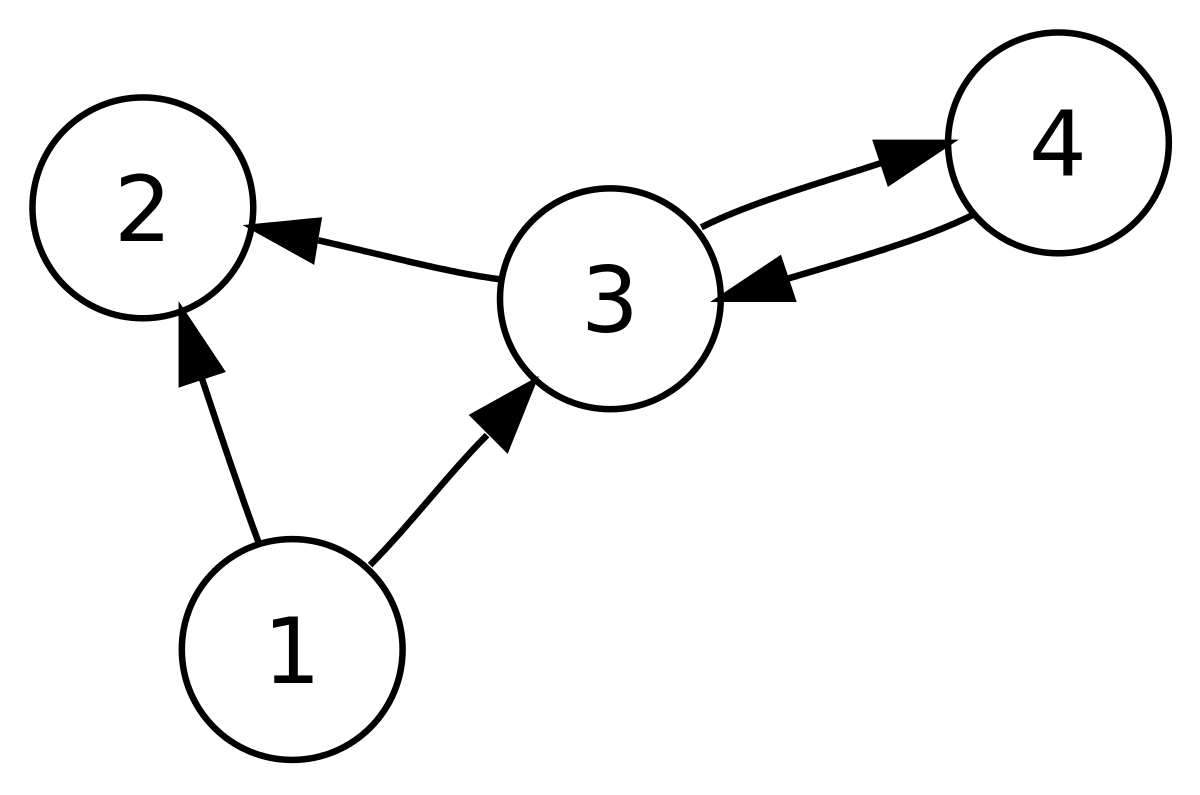
\includegraphics[width=0.5 \textwidth]{Figures/grapheOriente.png}
    \caption{Graphe non Orienté}
    \label{fig:Graphe Orienté}
\end{figure}

\end{frame}